\documentclass[11pt]{article}

\usepackage{maiacustom}

\begin{document}

\psettitle{Banco de questões de astronomia}

Estas questões foram produzidas/selecionadas cuidadosamente com o objetivo de preparar os estudantes para o processo seletivo de astronomia no Brasil. Algumas questões não são de autoria própria e estão devidamente sinalizadas por () antes do enunciado. O template do banco de questões é o mesmo do Professor \text{Kevin Zhou}. Seu trabalho é valioso, e diversas ideias desta lista podem ser encontradas em seus Handouts.

% \begin{psidea}{Título da Ideia}{}
% Ideia
% \end{psidea}

% \begin{psexample}{Título do Exemplo}{}
% Exemplo
% \end{psexample}

% \begin{pssolution*}{}{}
% Solução
% \end{pssolution*}

% \begin{psremark*}{Título da Observação}{}
% Observação
% \end{psremark*} 
\section{Óptica e Telescópios}

\pts{3}
    \begin{pproblem} Um telescópio Kepleriano possuí duas lentes convergentes. A primeira possuí o raio de curavtura das duas faces igual a \(R = 2\text{ m}\) e a segunda possuí ambos os raios de curvatura igual a \(r = 0,5 \text{ m}\). Considerando que ambas as lentes possuem espessura desprezivel e são feitas de um material com indíce de refração \(n=1,4\). Calcule o diâmetro e o aumento do telescópio sabendo que este telescópio é um f/12.
    \end{pproblem}

\pts{5}
    \begin{pproblem}
        Nessa questão, vamos nos familiarizar com uma das ferramentas mais poderosas da óptica, a \textit{óptica geométrica}. O objetivo dessa ferramenta é modelar lentes e espelho em forma de matrizes. Isso é muito útil para resolver questões envolvendo associações de diversas lentes e é um método de resolver problemas de óptica geométrica (praticamente) sem usar geometrica. Mas para isso, se atente as seguintes definições na imagem a seguir

        \begin{figure}[H]
            \centering
            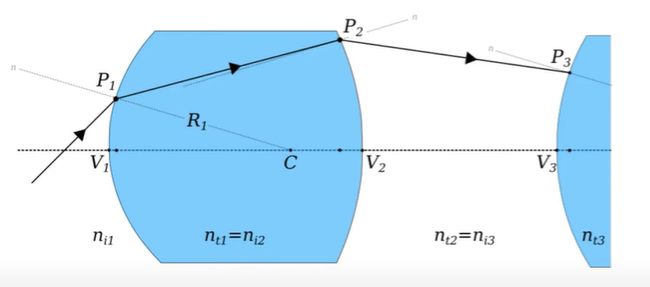
\includegraphics[width=0.9\linewidth]{imagens/lentes1.png}
            \caption{Esquema 1}
        \end{figure}

        Todas as linhas pontilhadas são paralelas ao eixo óptico, representado pela seta horizontal. É denotado por \(P_k\) o ponto onde a luz passa de um meio para o outro, \(y_k\) a coordenda vertical do ponto \(P_k\). São utilizados os subscritos \(i\) e \(t\) para se referir a incidente e transmitido, reespectivamente, então, por exemplo, \(\alpha_{i,k}\) é o ângulo que o raio de incidente luz faz com a horizontal no ponto \(P_k\), já o ângulo \(\alpha_k\) é o ângulo entre o ponto \(P_k\) e o centro da lente \(k\). Por exemplo, na figura, o ângulo \(\alpha_1\) é repsetenado por \(V_1\hat{C}P_1\).
        

        Para essa questão, vamos considerar que todos os ângulos de interesse são pequenos, de modo que \(\tan\theta \approx \sin\theta \approx \theta\).
        \begin{alternativas}
            \item Partindo da Lei de Snell, encontre uma relação entre \(n_{i,1}\), \(n_{t,1}\), \(\alpha_1\), \(\alpha_{i,1}\) e \(\alpha_{t,1}\).
        
            \item Encontre uma relação para \((1) \ n_{t,1}\alpha_{t,1}\) e \((2) \ y_{t,1}\). Deixe suas respostas em função de \(n_{i,1}\), \(\alpha_{i,1}\), \(y_{i,1}\) e \(\mathcal{D}_1\), para
            \[\mathcal{D}_1 = \frac{n_{t,1}-n_{i,1}}{R_1}\]

        Agora vamos para mais uma definição, seja o vetor \(\mathbf{r}_{t,1}= (n_{t,1}\alpha_{t,1}, \ y_{t,1})\) e \(\mathbf{r}_{i,1}= (n_{i,1}\alpha_{i,1}, \ y_{i,1})\).
        
            \item É possível escrever as duas equações que encontramos no item anterior na forma matricial, de forma:
            \[\mathbf{r}_{t,1}=\mathcal{R}_1\mathbf{r}_{i,1}\]
            Encontre a matriz \(2\times 2\) equivalente à \(\mathcal{R}_1\).

        Nosso interesse agora é encontrar as relações entre os pontos \(P_2\) e \(P_1\).

            \item Encontre uma equação para \(n_1\alpha_{i,2}\) e \(y_{i,2}\). Utilizando o raciocínio do item anterior, deixe sua resposta na forma
            \[\mathbf{r}_{i,2}=\Gamma_{2,1}\mathbf{r}_{t,1}\]
            Onde \(\Gamma_{2,1}\) também é uma matriz \(2\times 2\). Deixe sua resposta em função da espessura da lente, \(d_{2,1}\).

            \item Definimos a matriz da lente, \(\mathcal{A}_{2,1}\) da seguinte equação:
            \[\mathbf{r}_{t,2} = \mathcal{A}_{2,1}\mathbf{r}_{i,1}\]
            De modo que

            \[\mathcal{A}_{2,1} = \begin{pmatrix}
                a_{11} & a_{12} \\
                a_{21} & a_{22} \\
            \end{pmatrix}\]

            Encontre explicitamente \(\mathcal{A}_{2,1}\). Isso é de extrema importancia, pois descreve o raio de luz que sai da lente em função do raio que entra.

            \item Dentre todas as propriedades da matriz da lente, a mais curiosa delas é que o termo \(a_{12}\) é proporcional a \(-1/f\) onde \(f\) é o foco da lente. Prove esse resultado. (Dica: você consiguira escrever \(-a_{12}\) com uma equação bem conhecida da óptica).
        
        Agora, vamos colocar a mão na massa e fazer utilizações praticas da óptica matricial.

            \item Refaça o exercício anterior utilizando óptica matricial.
        
            \item Considere o seguinte esquema:
                \begin{figure}[H]
                    \centering
                    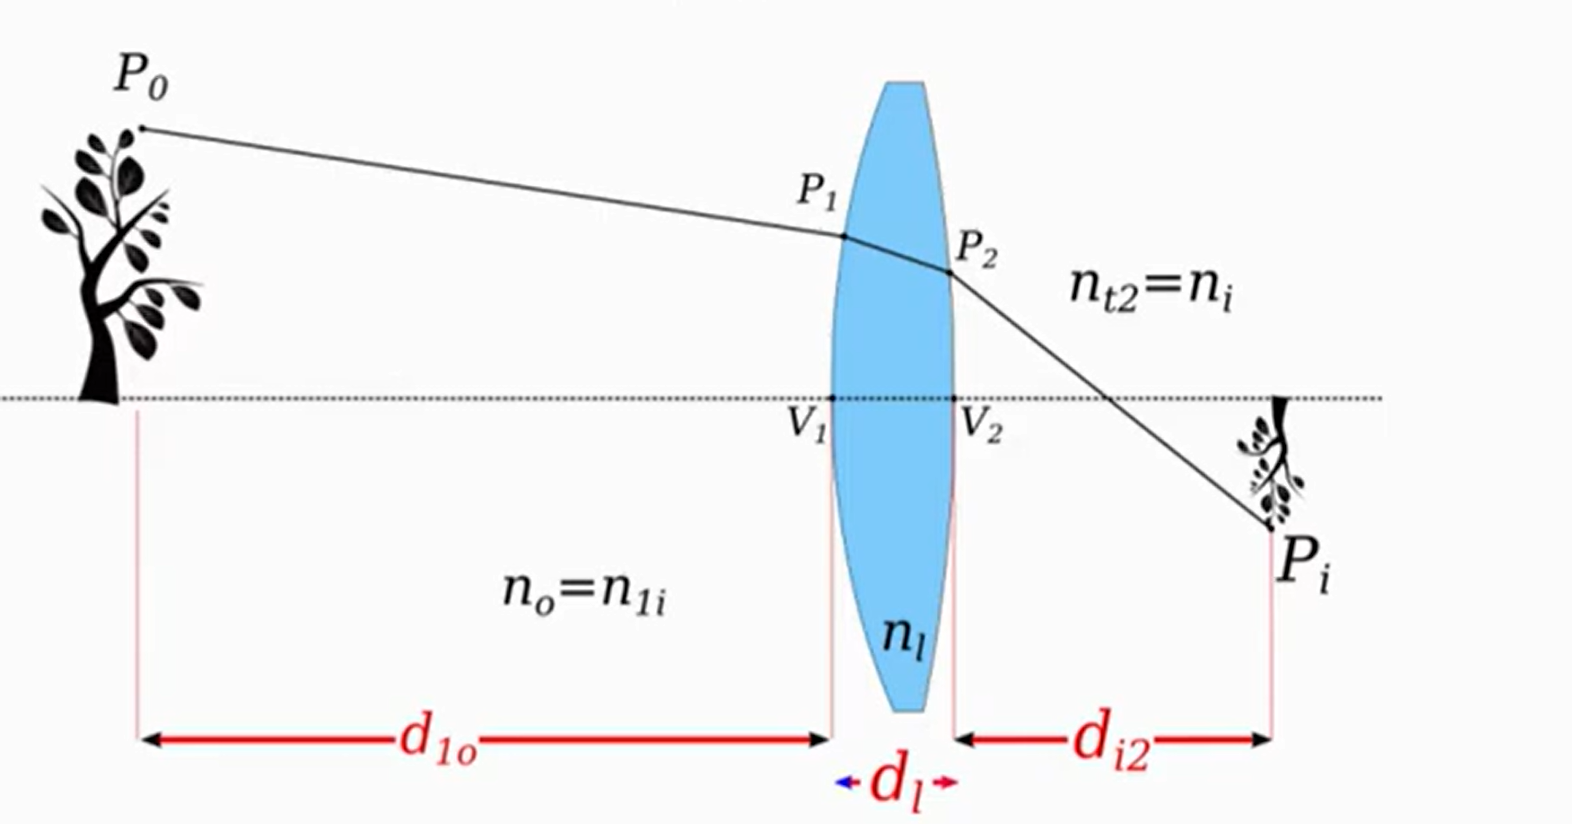
\includegraphics[width=0.9\linewidth]{imagens/lentes2.png}
                    \caption{Esquema 2}
                \end{figure}
                 Ecnontre \(y_i\) em função de \(y_0\) e dos dados na imagem.
                 
            \item Se a lente estiver entre dois meios diferentes, \(n_{i,1} \ne n_{t,2}\) temos a seguinte relação:
            \[a_{12} = -\frac{n_{i,1}}{f_0}=-\frac{n_{t,2}}{f_I}\]
                Utilizando-se disse, refaça a questão anterior, considerando que entre as duas lentes á água de \(n_w = 4/3\).
        
            \item Um arranjo muito comum de lentes é a Objetiva de Tessar, presente em muitas cameras pela sua eficiencia em diminuir efeitos de aberração e astigmatismo. O Arranjo tem a seguinte forma:
                \begin{figure}[H]
                    \centering
                    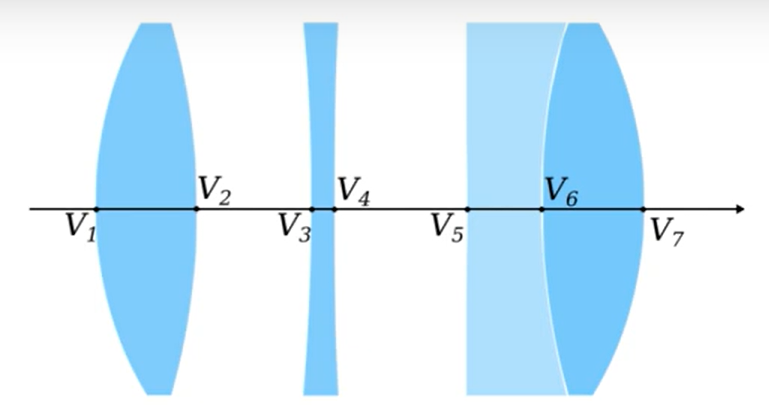
\includegraphics[width=0.7\linewidth]{imagens/lentes3.png}
                    \caption{Esquema Objetiva Tessar}
                \end{figure}
                Encontre a Matrix da Lente equivalente, \(\mathcal{A}_{1,7}\) em função de \(\mathcal{R}_i\) e \(\Gamma_{i,j}\).
        \end{alternativas}
    

\end{pproblem}

\pts{2}
\begin{pproblem}
    A teoria ondulatória da luz demonstra que um foco perfeito não é possível devido aos efeitos de difração associados à abertura finita da lente. Essa falta de foco perfeito impede que objetos muito próximos sejam distinguidos. Este problema pode ser estudado de dois pontos de vista diferentes:

    A teoria ondulatória da luz prevê que uma lente de diâmetro $D$ não pode focar um feixe paralelo de luz com comprimento de onda $\lambda$ em um ângulo menor que o limite de difração:
    \begin{equation}
        \theta_m \approx 1.22 \frac{\lambda}{D}
    \end{equation}

    Considere agora uma abordagem quântica, os fótons que são focados pela lente. Esses fótons são conhecidos por terem passado em algum lugar dentro de um raio do centro da lente. A incerteza na posição $x$ está associada a uma incerteza no componente $x$ do momento do fóton. Consequentemente, um fóton que, na ausência dessa incerteza, teria sido trazido para o eixo óptico do plano focal, pode agora ser desviado por um ângulo $\theta \ll 1$.

    Considere o comprimento de onda de de Broglie $\lambda = \frac{h}{p}$. Encontre um limite para $\theta$.

    \textbf{DICA:} o princípio de incerteza de Heisenberg, relaciona a impressição entre as medidas de momento e posição de uma particula por 
    \[\Delta p_x \Delta x = \frac{\hbar}{2}\]


\end{pproblem}

\pts{3}
\begin{pproblem} (Apostila Magna)
    Prove que a quantia \(n_iR_i\sin \theta_i\) para cascas esféricas adjacentes entre si, em que \(n_i\) é o índice de refração da i-ésima casca esférica, \(\theta_i\) é o ângulo que o raio de luz faz com a normal da i-ésima casca esférica e \(R_i\) é o raio da i-ésima casca esférica, é uma invariante
    
\end{pproblem}

\pts{4}
\begin{pproblem}
    O indídice de refração da atmosfera de um planeta é dado por, 

    \[n(h) = \frac{n_0}{1+\epsilon h}\]

    Onde \(n_0\) e \(epsilon\) são constantes.

    \begin{alternativas}
        \item Um raio de luz atinge a atmosfera paralelamente a superfície, há uma altura \(h'\ll R\), como será a trajetória?
        \item Sabendo a trajetória do raio de luz, calcule o Raio do planeta.
    
        \textbf{Dica:} Você pode achar útil a seguinte relação, 

        \[\int \frac{t}{\sqrt{a-bt^2}}dt = -\frac{1}{b}\sqrt{a-bt^2}+C\]
    \end{alternativas}

\end{pproblem}

\end{document}